\documentclass[a4paper]{article}

%% Language and font encodings
\usepackage[english]{babel}
\usepackage[utf8x]{inputenc}
\usepackage[T1]{fontenc}
\usepackage{helvet}
%\usepackage[numbers]{natbib}
\usepackage[round]{natbib}
%% For citations with atuhor et al year, usehttps://www.overleaf.com/16365895fcrtzrvgdsvp
%% \usepackage[round]{natbib}
%% \bibliographystyle{abbrv} (optional)
%% \citealt{adams1995hitchhiker}
\usepackage{upgreek} %%% This enables non-italic greek letters.
%% The lowercase letters are named \upalpha, \upbeta, ... and so, and upercase are named \Upalpha, \Upbeta, ...
%% line thickness
\usepackage{soul} %% Highlight package
\usepackage{lineno} %% Add line numbers to the document

%% Sets page size and margins
\usepackage[a4paper,top=3cm,bottom=2cm,left=3cm,right=3cm,marginparwidth=1.75cm]{geometry}
\setlength{\arrayrulewidth}{0.5mm}
\setlength{\tabcolsep}{4pt}

\renewcommand{\arraystretch}{1.3}
\newcommand{\beq}{\begin{equation}}
\newcommand{\eeq}{\end{equation}}

%% Useful packages
\usepackage{amsmath}
\usepackage{graphicx}
\usepackage[colorinlistoftodos]{todonotes}
\usepackage[colorlinks=true, allcolors=blue]{hyperref}
\usepackage{array}
\usepackage{float}
\usepackage{appendix} 
\usepackage{multirow}
\usepackage[symbol]{footmisc}
\usepackage{setspace}
\usepackage{authblk} %%% Support for footnote style author/affiliation.
\usepackage{ctable}
\renewcommand{\thefootnote}{\fnsymbol{footnote}}
\renewcommand\Affilfont{\itshape\small}
\usepackage{comment}
\usepackage{subfig}  
\usepackage{subcaption}
\usepackage{indentfirst}
\usepackage{siunitx}
\usepackage{amssymb,stmaryrd}
\usepackage{bbold}

\title{SLH Formalism: Sourced Feedback of Optical Parametric Oscillator}
\author[1]{Antonio Cobarrubia}
\affil[1]{Department of Physics, San Diego State University, San Diego, CA 92182}

\date{}

\begin{document}

\maketitle

\doublespacing
\section{Introduction}
Here is an explanation of the composition rules of SLH and a simple example to go alongside with it. I still need to learn how to derive each SLH operation (in-progress), but here is a first look on what SLH formalism can do and how someone can apply it to basic circuits. The SLH triple for each individual component can be found through other methods, which we can use other methods/material to build the scattering matrix, coupling operator and hamiltonian. From there SLH can be applied. 

\section{Basic Algebraic Rules of SLH}
The SLH composition rules are algebraic descriptions of combining components in various manners, under asymptotic free fields approximation. These rules will give us insight on how to evaluate (optical) circuit components. 
\section*{Series Product} 

\begin{figure}[H]
\centering
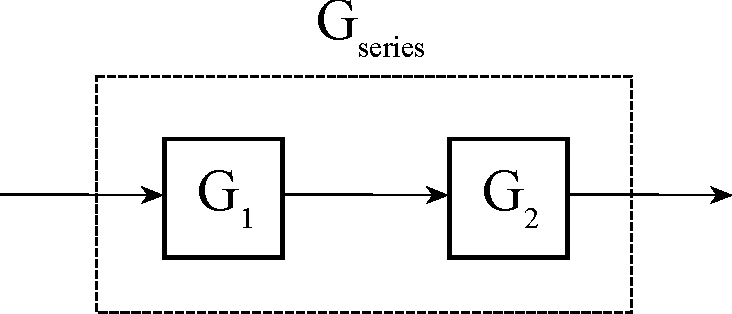
\includegraphics[width = 7.5 cm]{Series_Product.pdf}
\caption{Series of component $G_1$ output is cascaded into the input of $G_2$.
}
\label{fig:series}
\end{figure}  

For two components connected in series, where the output goes from $G_1$ = ($S_1,L_1,H_1$) to the input of $G_2 = (S_2, L_2, H_2)$ is defined as a series product (cascade rule), as seen in Figure \ref{fig:series}. The ith number of inputs/outputs in $G_1$ have to be the same as the jth input/output of $G_2$. In particular, this connection is directional, where the series product ($\triangleleft $) is not equivalent if the output of 2 goes into the input of 1. The connection is given by 

\begin{align*}
    G_{\text{series}} = & \ G_2 \triangleleft G_1 \\
    G_{\text{series}} = & \ (\textbf{S}_2,\textbf{L}_2,H_2) \triangleleft (\textbf{S}_1,\textbf{L}_1,H_1)
\end{align*}
\begin{align}
    G_{\text{series}} = & \ \Bigg( \textbf{S}_2\textbf{S}_1,\textbf{L}_2+\textbf{S}_2\textbf{L}_1,H_1 + H_2 + \frac{1}{2i}(\textbf{L}_2^\dagger \textbf{S}_2\textbf{L}_1 - \textbf{L}_1^\dagger \textbf{S}_2^\dagger \textbf{L}_2) \Bigg)
    \label{eq:series}
\end{align}


\section*{Concatenation Product}

\begin{figure}[H]
\centering
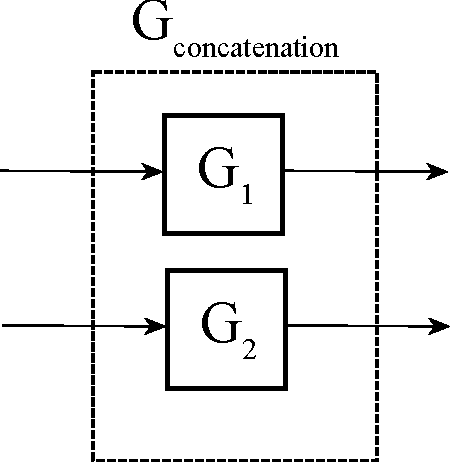
\includegraphics[width = 7.5 cm]{Concatenation_product.pdf}
\caption{A parallel connection known as a concatenation product of $G_1$ and $G_2$.
}
\label{fig:concatenation}
\end{figure}  

Components that are grouped in parallel is denoted as the concatenation product ($ \boxplus $) as seen in Figure \ref{fig:concatenation}. This connection is more universal, where a component direction isn't localized like the series product. The following connection is defined by

\begin{align*}
    G_{\text{concatenation}} = & \ G_1 \boxplus G_2 \\
    G_{\text{concatenation}} = & \ (\textbf{S}_1,\textbf{L}_1,H_1) \boxplus (\textbf{S}_2,\textbf{L}_2,H_2)
\end{align*}
\begin{align}
    G_{\text{concatenation}} = & \ \Bigg( \begin{pmatrix} \textbf{S}_1 & 0 \\ 0 & \textbf{S}_1\end{pmatrix},\begin{bmatrix} \textbf{L}_1 \\ \textbf{L}_2 \end{bmatrix},H_1 + H_2 \Bigg)
    \label{eq:concatenation}
\end{align}


\section*{Direct Coupling}

\begin{figure}[H]
\centering
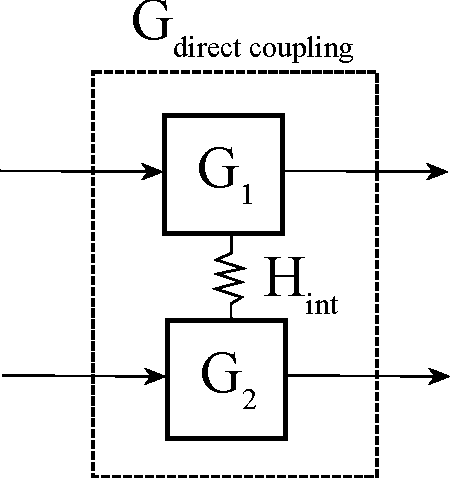
\includegraphics[width = 7.5 cm]{Direct_coupling.pdf}
\caption{Parallel connection with direct coupling of some interaction hamiltonian $H_{\text{int}}$ between $G_1$ and $G_2$. 
}
\label{fig:direct_coupling}
\end{figure}  

This connection is a special rule of a concatenation product, where there is direct coupling ($\bowtie$) between two components, as shown in Figure \ref{fig:direct_coupling}. The same method of concatentaion product applies to direct coupling, but with an additional interaction hamiltonian. This connection is given by 

\begin{align*}
    G_{\text{direct coupling}} = & \ G_1 \bowtie G_2 \\
    G_{\text{direct coupling}} = & \ (\textbf{S}_1,\textbf{L}_1,H_1) \bowtie (\textbf{S}_2,\textbf{L}_2,H_2)
\end{align*}
\begin{align}
    G_{\text{direct coupling}} = & \ \Bigg( \begin{pmatrix} \textbf{S}_1 & 0 \\ 0 & \textbf{S}_1\end{pmatrix},\begin{bmatrix} \textbf{L}_1 \\ \textbf{L}_2 \end{bmatrix},H_1 + H_2 + H_{\text{int}} \Bigg)
    \label{eq:direct_coupling}
\end{align}

Note: The previous rules were derived with a vacuum source term using weak coupling approximations like the rotating wave approximation. The direct coupling rule will help construct more complicated systems using simple algebraic operations.

\section*{Feedback Reduction}

\begin{figure}[H]
\centering
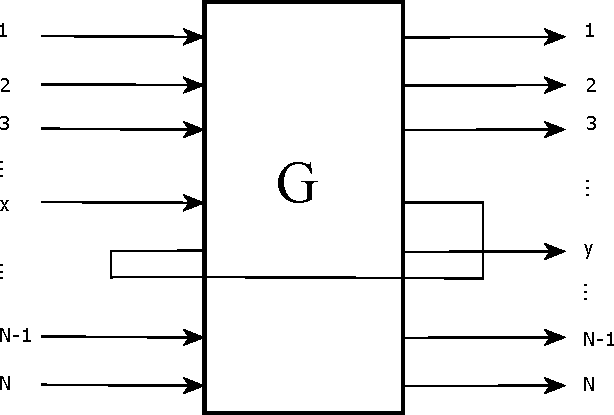
\includegraphics[width = 7.5 cm]{Feedback.pdf}
\caption{A cascaded system where the output of one port is connected to the input of another in the same component.
}
\label{fig:feedback_reduction}
\end{figure}  
The feedback reduction rule is a special rule for cascaded systems, shown in Figure \ref{fig:feedback_reduction}. This rule is a derivative of the series product by splitting a component with N amount of ports into Nth amount of individual components, and connecting the xth output port to the yth input port. The symbol of such rule is denoted as x $ \rightarrow $y. For individual components connected in a feedback reduction loop as seen in Figure \ref{fig:circuit}(a), all components are treated as an unconnected concatenation product then the reduction feedback rules apply to this unconnected form. The resulting connection is defined as 

\begin{align*}
    G_{x \rightarrow y} = & \ \Bigg( \textbf{S}_{\text{reduction}}, \textbf{L}_{\text{reduction}}, H_{\text{reduction}} \Bigg) \\
\end{align*}
\begin{align}
\textbf{S}_{\text{reduction}} = & \ \textbf{S}_{\Bar{x}\Bar{y}} + \textbf{S}_{\Bar{x}y}(\mathbb{1}_{reduced}-S_{(x,y)})^{-1}\textbf{S}_{x\Bar{y}} \\
\textbf{L}_{\text{reduction}} = & \ \textbf{L}_{\Bar{x}}+\textbf{S}_{\Bar{x}y}(\mathbb{1}_{reduced}-S_{(x,y)})^{-1}L_{(x)} \\
H_{\text{reduction}} = & \ H + \frac{1}{2i}(\textbf{L}^\dagger \textbf{S}_{:,y}(\mathbb{1}_{reduced}-S_{(x,y)})^{-1}L_{(x)} - L_{(x)}^\dagger (\mathbb{1}_{reduced}-S^\dagger_{(x,y)})^{-1}\textbf{S}^\dagger_{:,y}\textbf{L}) 
    \label{eq:feedback}
\end{align}
where $\textbf{S}_{\Bar{x}\Bar{y}} $ is the \textbf{S} matrix without the x row; $\textbf{S}_{\Bar{x}y}$ is the yth column of the \textbf{S} matrix without the x row (visa versa with $\textbf{S}_{x\Bar{y}}$); $S_{(x,y)}$ is the xth and yth component of the \textbf{S} matrix; $\textbf{S}_{:,y}$ is the entire yth column of the \textbf{S} matrix; $\textbf{L}_{\Bar{x}}$ is the \textbf{L} vector without the xth row; $L_x$ is the x component of the \textbf{L} vector. The identity matrix $\mathbb{1}_{reduced}$ in the reduced SLH, has dimensions of the reduced Hilbert space.

\section{ Non-vacuum Sourced States: Flock States}

\begin{figure}[H]
\centering
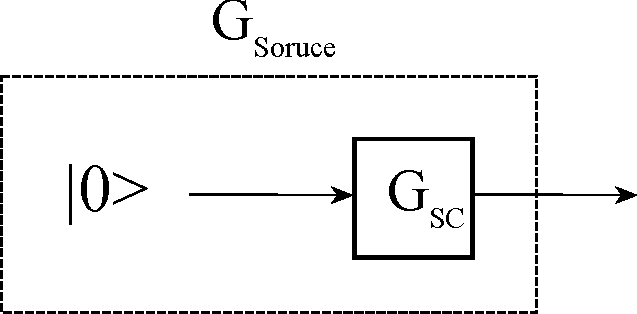
\includegraphics[width = 7.5 cm]{Soruce_term.pdf}
\caption{Non-vacuum sourced SLH model based on Fock states.
}
\label{fig:soruced_term}
\end{figure}  
SLH formalism is derived on the assumption of a vacuum input, which isn't ideal for most cases. Additional models that examine arbitrary photon input states are needed to develop SLH as seen in Figure \ref{fig:soruced_term}. One way is by proposing the source term to be coupled with a vacuum state that is fed into a sourced SLH triple for continuous-mode of coherent photons, also known as Fock states. A general case is given by  

\begin{align}
    G_{\text{Flock}} = & \ (\mathbb{1}, \lambda(t)a,0); \ \rho_{source}(t=0)= |n><n|
    \label{eq:sourced_term}
\end{align}
where a is an arbitrary system operator, $|n>$ are eigenstates of the probability density matrix, and $\lambda$ is defined as 

\begin{align*}
    \lambda(t) = \frac{\zeta(t)}{\sqrt{A(t)}} ; \ A(t) = \int_{t}^{\infty} ds |\zeta(s)|^2.
\end{align*}
For Fock states $\zeta(t)$ is the spectral density function.  
\section{EXAMPLE: Sourced Feedback of Optical Parametric Oscillator}


\begin{figure}[H]
\centering
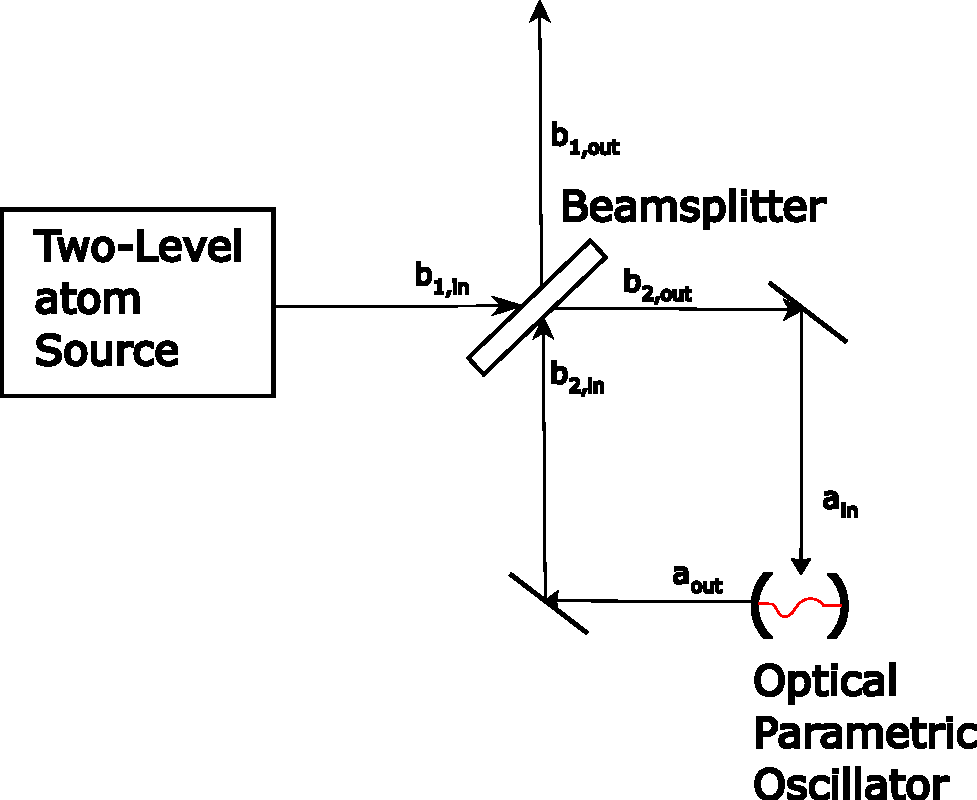
\includegraphics[width = 7.5 cm]{Example_Sourced_feedback.pdf}
\caption{Full circuit schematic of a sourced-optical parametric oscillator feedback system.
}
\label{fig:Example}
\end{figure}  

Here I have devised a simple circuit that combines the all of the basic rules (except direct coupling) and a Fock state sourced component, Figure \ref{fig:Example}. This example should highlight how to tackle the most complicated rule, the feedback reduction, alongside the concatenation and series product. The example consist of a two-level atom source with a gaussian spectral distribution ($G_{\text{Source}} $) is then pumped into the circuit component ($G_{\text{Circuit}})$ as seen in Figure \ref{fig:SLH_form}(a), which is composed of an optical parametric oscillator ($G_{text{OPO}}$) in a feedback loop with a beamsplitter ($G_B$) ($b_{2,out}$ = $a_{in}$ and $b_{2,in} = a_{out}$). Each SLH triple is defined as 

\begin{align*}
    G_{\text{Source}} = & \ ((\mathbb{1}, \lambda(t) \sigma_-,0)); \ \zeta(t)  = (\frac{\Omega^2}{2\pi})^{\frac{1}{4}}e^{\frac{-\Omega^2}{4}(t-t_c)^2} \\
    G_{\text{B}} = & \ \Bigg( \begin{pmatrix} -\sqrt{1-\eta^2} & \eta \\ \eta & \sqrt{1-\eta^2} \end{pmatrix},\begin{bmatrix} 0 \\ 0\end{bmatrix}, 0 \Bigg) \\ 
    G_{OPO} = & \ (\mathbb{1}, \sqrt{\kappa}a, i\epsilon(a^\dagger a^\dagger - a a))
\end{align*}
where $\sigma_-$ is the lowering atomic transition operator, $\Omega$ and $t_c$ are parameters for a guassian wave packet, $\eta$ is the transmission coefficient, $\kappa$ the decay rate of a photon in an optical parametric oscillator, and a is the bosonic annihilation operator for the optical parametric oscillator. The initial probability density starts at an excited state ($\rho_{source}$ = |$N_{\text{Fock}}$><e|). 
\begin{figure}[H]
\centering
   \subfloat[Broken Schematic based on Source-Circuit components.]{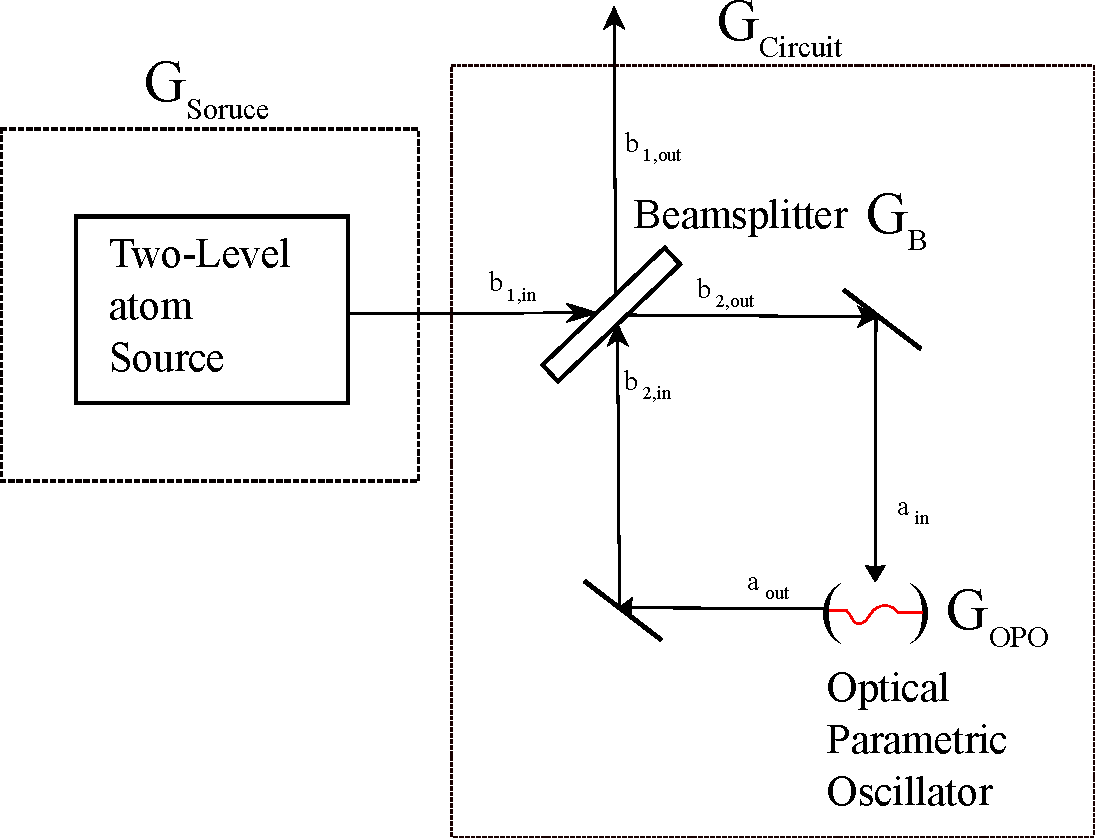
\includegraphics[width= 7.5 
   cm,keepaspectratio]{Example_Sourced_feedback2.pdf}}
     \hspace{2cm}
     \subfloat[SLH equivalent schematic.]{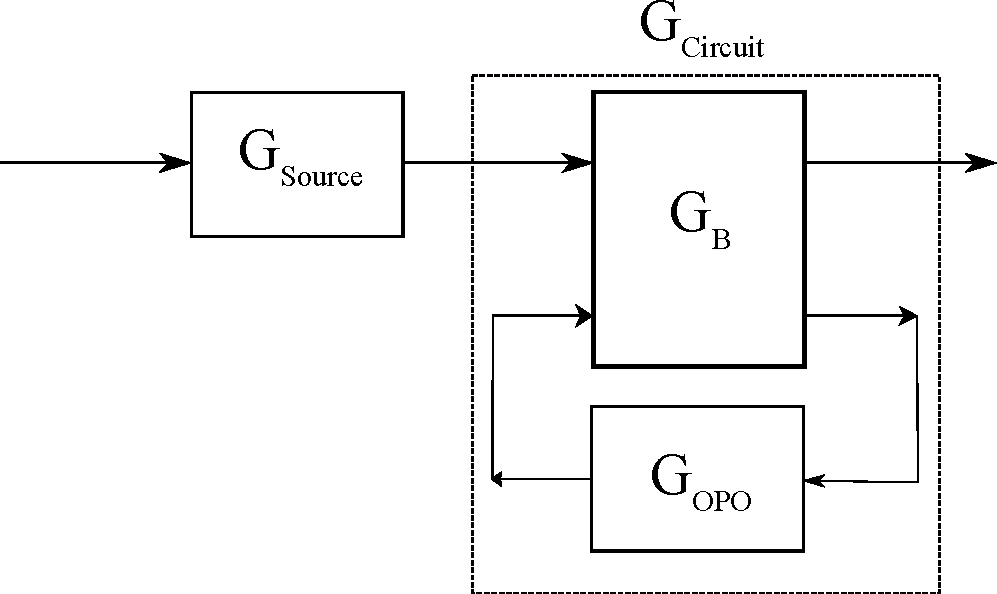
\includegraphics[width= 7.5 cm,keepaspectratio]{Example_Sourced_feedback_SLH.pdf}}

     \caption{Breakdown of a sourced-optical parametric oscillator feedback system into SLH form. The names of each component is associated with their SLH triple: Source ($G_{\text{Source}}$), beamsplitter ($G_{\text{B}}$), Optical Parametric Oscillator ($G_{\text{OPO}}$), equivalent circuit component ($G_{\text{Circuit}}$). (a) The physical system schematic. (b) The SLH equivalent of the system.}
     \label{fig:SLH_form}
\end{figure}     

NOTE: The local dimensions of the scattering matrix is the number of ports for the component. For example, the source term only has one port while the beamsplitter has two even though the identity has m by m dimensions based on the hilbert space of the sourced component. This leads to a possibility (not mentioned in any SLH paper) that we can split up a component into numerous amount of ports based on a components Hilbert space.

\section*{Sourced Component}
Following up with the sourced component (left, Figure \ref{fig:SLH_form}(b)), we then can use eq. \ref{eq:sourced_term} for a two level atom to construct an arbitrary input state. The normalization of the spectral density function A(t) is defined as 

\begin{align*}
    A(t) = & \int_{t}^{\infty} ds |(\frac{\Omega^2}{2\pi})^{\frac{1}{4}}e^{\frac{-\Omega^2}{4}(s-t_c)^2}|^2  = \frac{1}{2}(erfc(\frac{\sqrt{2}\Omega(t_c-t)}{2}+1).
\end{align*}
Thus, we can then define the time dependent dissipate term ($\lambda$(t)):

\begin{align*}
    \lambda(t) = & \ (\frac{\Omega^2}{2\pi})^{\frac{1}{4}}\frac{e^{\frac{-\Omega^2}{4}(s-t_c)^2}}{ \sqrt{\frac{1}{2}(erfc(\frac{\sqrt{2}\Omega(t_c-t)}{2}+1)}}
\end{align*}
For a two-level atom, the lower atomic transition operator is defined as
\begin{align*}
    \sigma_- =& \ \begin{pmatrix} 0 & 1 \\ 0 & 0 \end{pmatrix}
\end{align*}
The extension of a fock state input states that our initial state of $\rho_{SC}(0) = |N_{\text{Fock}}><e|$, where |e> is the excited state of the two-level atom. Based on all of this information, we can then construct the input SLH triple. 

\begin{align}
    G_{SC} = & ( \mathbb{1}, \lambda(t)\sigma_-, 0) ; \ \rho_{SC}(0) = |N_{\text{Fock}}><e|
    \label{eq:EX_source}
\end{align}
\section*{Circuit Component}
\begin{figure}[H]
\centering
   \subfloat[Reduction of circuit by $G^{1 \rightarrow 2}_{\text{unconnected}}$.]{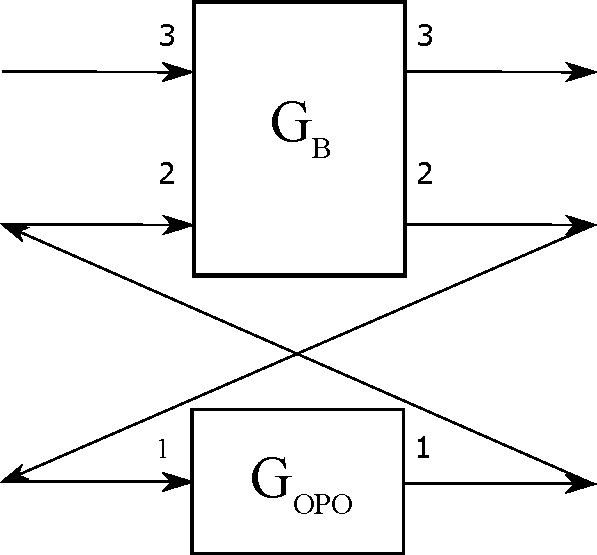
\includegraphics[width= 4 
   cm,keepaspectratio]{EX_reduction1.pdf}}
     \hspace{2cm}
     \subfloat[Reduction of circuit by $G^{1 \rightarrow 1}_{\text{B-OPO}}$.]{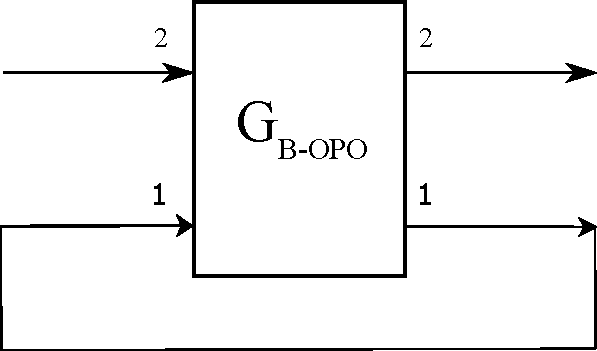
\includegraphics[width= 4 cm,keepaspectratio]{EX_reduction2.pdf}}

     \caption{Simplification of circuit component through feedbackreduction. (a) After concatenation product of unconnected beamsplitter and OPO, the output port 1 is fed into input port 2 labeled in the figure. (b) Redefining the ports as specified in Figure \ref{fig:circuit}(b), the new reduced circuit  component $G_{\text{B-OPO}}$ under goes another feedback reduction from output port 1 to input port 1.}
     \label{fig:circuit}
\end{figure}     
Now, we can simplify all of the circuit components into an equivalent SLH triple $G_{\text{Circuit}}$ which will then be in a series with the source component, Figure \ref{fig:Final_connection}. First, we need to reduced the feedback of output port 1 to input port 2 as described in Figure \ref{fig:circuit}(a) using the rules of eq. \ref{eq:feedback}. The order of reduction doesn't matter. We could have started with $2 \rightarrow 1$ instead of $1 \rightarrow 2$. I chose to reduce $1 \rightarrow 2$ first. This is done by first setting up a concatenation product of the two components as if they were unconnected.
\begin{align*}
    G_{\text{unconnected}} = & \ G_{OPO}  \boxplus G_B \\
    G_{\text{unconnected}} = & \  (\mathbb{1}, \sqrt{\kappa}a, i\epsilon(a^\dagger a^\dagger - a a))   \boxplus \Bigg( \begin{pmatrix} -\sqrt{1-\eta^2} & \eta \\ \eta & \sqrt{1-\eta^2} \end{pmatrix},\begin{bmatrix} 0 \\ 0\end{bmatrix}, 0 \Bigg)
\end{align*}
We can apply the concatenation rules from eq. \ref{eq:concatenation} to get the following result
\begin{align*}
     G_{\text{unconnected}} = & \ \Bigg( \begin{pmatrix} \mathbb{1} & 0 & 0 \\ 0 & -\sqrt{1-\eta^2} & \eta \\ 0 & \eta & \sqrt{1-\eta^2}  \end{pmatrix},\begin{bmatrix} \sqrt{\kappa}a \\ 0 \\ 0 \end{bmatrix}, H_{OPO} \Bigg).
\end{align*}
Now, we need to connect the output port 1 to input port 1 by applying eq. \ref{fig:feedback_reduction} as follows, where x = 1, y = 2, and $\mathbb{1}_{reduced} = \mathbb{1}_2$: 
\begin{align*}
    G_{\text{unconnected}}^{1 \rightarrow 2} = & \ (S_{1 \rightarrow 2}, L_{1 \rightarrow 2}, H_{1 \rightarrow 2}) =  G_{\text{B-OPO}} &  \\
    S_{1 \rightarrow 2} = & \ \begin{pmatrix}  0 & \eta \\ 0 & \sqrt{1-\eta^2}  \end{pmatrix} + \begin{bmatrix}  -\sqrt{1-\eta^2} \\ \eta \end{bmatrix} (\mathbb{1}_2-0)^{-1} \begin{bmatrix} \mathbb{1}  & 0 \end{bmatrix} & \\
    L_{1 \rightarrow 2} = & \ \begin{bmatrix}  0 \\ 0 \end{bmatrix} + \begin{bmatrix}  -\sqrt{1-\eta^2} \\ \eta \end{bmatrix} (\mathbb{1}_2-0)^{-1}(\sqrt{\kappa}a) & \\
    H_{1 \rightarrow 2} = & \ H_{OPO} + \frac{1}{2i}\Bigg( \begin{bmatrix} \sqrt{\kappa}a^\dagger  & 0 & 0 \end{bmatrix} \begin{bmatrix} 0   \\  -\sqrt{1-\eta^2} \\ \eta \end{bmatrix}  (\mathbb{1}_2)^{-1}(\sqrt{\kappa}a) \ - &  
    \\ &  (\sqrt{\kappa}a^\dagger) (\mathbb{1}_2)^{-1} \begin{bmatrix} 0  &  - \sqrt{1-\eta^2} & \eta \end{bmatrix} ) \begin{bmatrix} \sqrt{\kappa}a \\ 0 \\ 0 \end{bmatrix} \Bigg)
\end{align*}

Note:  $\mathbb{1}^{-1}_2 = \mathbb{1}_2$, and anything multiplied by the identity is itself. Notice that the reduced hamiltonian is just $H_{OPO}$. Thus, the result of the first feedback reduction as shown in Figure \ref{fig:circuit}(b) is given by 
\begin{align}
    G_{\text{B-OPO}} = & \ \Bigg( \begin{pmatrix} -\sqrt{1-\eta^2} & \eta \\ \eta & \sqrt{1-\eta^2} \end{pmatrix}, \begin{bmatrix}  -\sqrt{1-\eta^2}(\sqrt{\kappa}a) \\ \eta(\sqrt{\kappa}a) \end{bmatrix}, H_{OPO}  \Bigg)
    \label{eq:EX_reduced_1}
\end{align}
Finally, we can do one more feedback reduction to obtain the equivalent circuit SLH triple. Redefining the port as described in Figure \ref{fig:circuit}(b), we'll do a feedback reduction of $1 \rightarrow 1$ using eq. \ref{eq:feedback} with x = 1 and y = 1, and the new reduced identity $\mathbb{1}_{reduced} = 1$. We'll use the result obtained in eq. \ref{eq:EX_reduced_1} as shown in Figure \ref{fig:circuit}(b).
\begin{align*}
    G_{\text{B-OPO}}^{1 \rightarrow 1} = & \ (S_{1 \rightarrow 1}, L_{1 \rightarrow 1}, H_{1 \rightarrow 1}) =  G_{\text{Circuit}} & \\
    S_{1 \rightarrow 1} = & \ \sqrt{1-\eta^2} + \eta (1+\sqrt{1-\eta^2})^{-1}(\eta)& \\
    L_{1 \rightarrow 1} = & \ \eta(\sqrt{\kappa}a) + \eta (1+\sqrt{1-\eta^2})^{-1}(-\sqrt{1-\eta^2}(\sqrt{\kappa}a)) & \\
    H_{1 \rightarrow 1} = & \ H_{OPO} + \frac{1}{2i}\Bigg( \begin{bmatrix} -\sqrt{1-\eta^2}\sqrt{\kappa}a^\dagger  & \eta \sqrt{\kappa}a^\dagger \end{bmatrix} \begin{bmatrix}   -\sqrt{1-\eta^2} \\ \eta \end{bmatrix}  (1+\sqrt{1-\eta^2})^{-1} ( -\sqrt{1-\eta^2}\sqrt{\kappa}a) \ - &  
    \\ &  ( -\sqrt{1-\eta^2}\sqrt{\kappa}a^\dagger) (1+\sqrt{1-\eta^2})^{-1} \begin{bmatrix}  - \sqrt{1-\eta^2} & \eta \end{bmatrix} ) \begin{bmatrix} -\sqrt{1-\eta^2}(\sqrt{\kappa}a) \\ \eta(\sqrt{\kappa}a) \end{bmatrix} \Bigg)& 
\end{align*}
After basic algebraic operations we'll arrive at the equivalent circuit SLH triple. 
\begin{align}
    G_{\text{Circuit}} = & \ \Bigg( \mathbb{1}, \ell \sqrt{\kappa}a ,H_{OPO}\Bigg); \ \ell = \frac{\eta}{(1+\sqrt{1-\eta^2})}
    \label{eq:Ex_Circuit}
\end{align}
\section*{Total SLH Triple}

\begin{figure}[H]
\centering
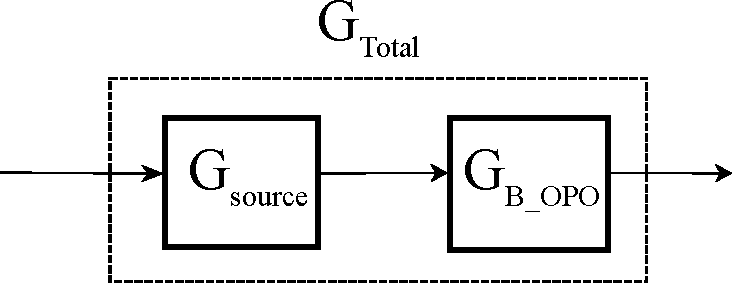
\includegraphics[width = 9 cm]{Example_Sourced_feedback_final.pdf}
\caption{Series product of the source term with the reduced $G_{\text{B-OPO}}$.
}
\label{fig:Final_connection}
\end{figure}  

We have broken down every component into two basic SLH triples: $G_{\text{Source}}$ and $G_{\text{Circuit}}$. Based on Figure \ref{fig:Final_connection}, we can use eq. \ref{eq:series} to get the total system SLH triple with eq. \ref{eq:EX_source} and \ref{eq:Ex_Circuit}. The final result is given by 
\begin{align*}
    G_{\text{Total}} = & \ G_{\text{Circuit}} \triangleleft G_{\text{SC}} \\
    G_{\text{Total}} = & \ \Bigg( \mathbb{1}, \ell \sqrt{\kappa}a ,H_{OPO}\Bigg) \triangleleft \Bigg( \mathbb{1}, \lambda(t)\sigma_-, 0 \Bigg) \\ 
    G_{\text{Total}} = & \ \Bigg( \mathbb{1}\mathbb{1}, \ell \sqrt{\kappa}a +  \mathbb{1} \lambda(t)\sigma_-,H_{OPO} + \frac{1}{2i}(\ell \sqrt{\kappa}a^\dagger \mathbb{1}  \lambda(t)\sigma_- - \lambda^*(t)\sigma_-^\dagger \mathbb{1}  \ell \sqrt{\kappa}a) \Bigg)
\end{align*}
\begin{align}
    G_{\text{Total}} = & \ \Bigg( \mathbb{1}, \ell \sqrt{\kappa}a + \lambda(t)\sigma_-, i\epsilon(a^\dagger a^\dagger - a a) + \frac{\ell \sqrt{\kappa}}{2i}(a^\dagger \lambda(t)\sigma_- - \lambda^*(t)\sigma_-^\dagger a) \Bigg)
    \label{eq:EX_FINAL_RESULT}
\end{align}

I hope this example is able to capture the core aspects of SLH formalism. As seen in this example, we can tackle difficult quantum based circuits using rudimentary, algebraic operations. In later examples, hopefully I'll be able to show you how to derive each SLH operation and explain more in detail. Alongside with this document, I'll have the jupyter notebook example that numerically solves the master equation using QuTip with this SLH triple. All rules were derived from Joshua Combes SLH tutorial ("The SLH framework for modeling quantum input-output networks"). 
\end{document}
